\documentclass[10pt,xcolor=pdflatex]{beamer}
\usepackage{newcent}
\usepackage[utf8]{inputenc}
\usepackage[czech]{babel}
\usepackage{hyperref}
\usepackage{fancyvrb}
\usetheme{FIT}

%%%%%%%%%%%%%%%%%%%%%%%%%%%%%%%%%%%%%%%%%%%%%%%%%%%%%%%%%%%%%%%%%%
\title[Distribuovaný repositář digitálních forenzních dat]{Distribuovaný repositář digitálních forenzních dat}

\author[]{Bc. Martin Josefík}

\institute[]{Vysoké učení technické v Brně, Fakulta informačních technologií\\
Božetěchova 1/2. 612 66 Brno - Královo Pole\\
xjosef00@fit.vutbr.cz}

%\date{January 1, 2016}
\date{\today}
%\date{} % bez data

%%%%%%%%%%%%%%%%%%%%%%%%%%%%%%%%%%%%%%%%%%%%%%%%%%%%%%%%%%%%%%%%%%

\begin{document}

%-------------------------------------
\frame[plain]{\titlepage}

%Na prezentaci je 10 minut + 5 minut otázky. Ve své prezentaci se zaměřte se na cíle své DP a splnění bodů v zadání, které se kontrolují u semestrálního projektu.
%-------------------------------------

\begin{frame}\frametitle{Cíl práce}
    \begin{block}{Teoretická část - Seznámení se s}
        \begin{itemize}
            \item Formáty digitálních forenzních dat
            \item Existujícími systémy pro jejich uložení
            \item Distribuovanými databázemi
        \end{itemize}
    \end{block}
    \begin{block}{Praktická část}
        \begin{itemize}
            \item Navržení distribuovaného úložiště
            \item Zvolení vhodných technologií
            \item Implementace
            \item Testy použití a výkonu
            \item Vyhodnocení
        \end{itemize}
    \end{block}
\end{frame}

%-------------------------------------

\begin{frame}\frametitle{Teoretická část}
%Seznamte se s formáty digitálních forenzních dat a způsoby jejich uložení. Prozkoumejte existující systémy pro uložení digitálních forenzních dat (např. AFF4). Seznamte se s distribuovanými databázemi a úložišti pro rozsáhlá strukturovaná i nestrukturovaná data.
%Navrhněte distribuované úložiště rozsáhlých digitálních forenzních dat (Big data) vč. aplikačního rozhraní pro optimální přístup k různým datům (sekvenční a náhodní čtení, dotazování, zpracování Big data přístupy). Zvolte vhodné technologie pro implementaci úložiště.
%Po konzultaci s vedoucím navržené úložiště implementujte. Úložiště musí umožňovat přidávání podpory pro nové druhy forenzních dat za běhu. Otestujte použití a výkon úložiště pro vybrané druhy digitálních forenzních dat.
%Výsledky zdokumentujte, vyhodnoťte a projekt zveřejněte jako open-source.
\begin{block}{Forenzní analýza digitálních dat}
    \begin{itemize}
        \item Cíl, průběh, vlastnosti
        \item Formáty digitálních forenzních dat
        \item Existující systémy (AFF4)
    \end{itemize}
\end{block}
\begin{block}{Úložiště pro strukturovaná a nestrukturovaná data}
    \begin{itemize}
        \item Big data
        \item Distribuované databáze
        \item Strukturovaná a nestrukturovaná data
    \end{itemize}
\end{block}
\end{frame}

%-------------------------------------

\begin{frame}\frametitle{Návrh systému}
\begin{block}{Požadavky}
    \begin{itemize}
        \item Distribuované úložiště
        \item Rozsáhlá digitální forenzní data
        \item Optimální přístup k datům
        \item Rozšiřitelnost pro nové druhy dat
    \end{itemize}
\end{block}
\begin{block}{Technologie}
    \begin{itemize}
        \item Kafka
        \item NoSQL databáze - Cassandra, MongoDB
        \item HDFS
    \end{itemize}
\end{block}
\begin{block}{Ovládání systému}
    \begin{itemize}
        \item Zasílání zpráv - příkazů
    \end{itemize}
\end{block}
\end{frame}

%-------------------------------------

\begin{frame}\frametitle{Komunikace s klientem}
\begin{figure}[!h]
  \centering
  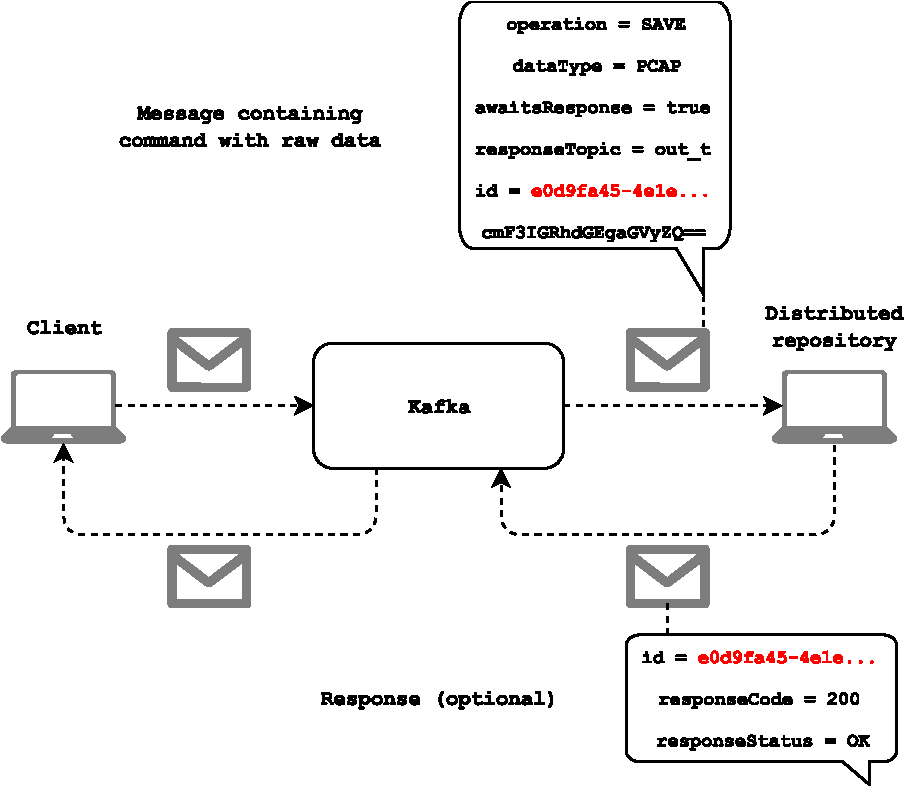
\includegraphics[width=9cm]{img/Kafka_communication.pdf}
  \label{FIG_KafkaCommunication}
\end{figure}
\end{frame}

%-------------------------------------

\begin{frame}\frametitle{Architektura}
\begin{block}{Zpracování zpráv}
    \begin{itemize}
        \item Přiřazení akce k příkazu
        \item Akce zapouzdřuje všechny potřebné operace
        \item Obsluha úložišť
    \end{itemize}
\end{block}
\begin{block}{Metadata}
    \begin{itemize}
        \item Registr dat
        \item Předzpracování dat
        \item Optimální přístup k datům
        \item Dynamičnost metadat
    \end{itemize}
\end{block}
\end{frame}

%-------------------------------------

\begin{frame}\frametitle{Úložiště}
\begin{block}{Strukturovaná data}
    \begin{itemize}
        \item Lze rozdělit na části, segmenty, bloky
        \item Před uložením serializována
        \item NoSQL databáze
    \end{itemize}
\end{block}
\begin{block}{Nestrukturovaná data}
    \begin{itemize}
        \item Logy, multimédia, ...
        \item Rozdělení a serializace dat brzdí výkon
        \item Distribuovaný souborový systém (HDFS)
    \end{itemize}
\end{block}
\end{frame}

%-------------------------------------

\begin{frame}\frametitle{Moduly}
\begin{figure}[!h]
  \centering
  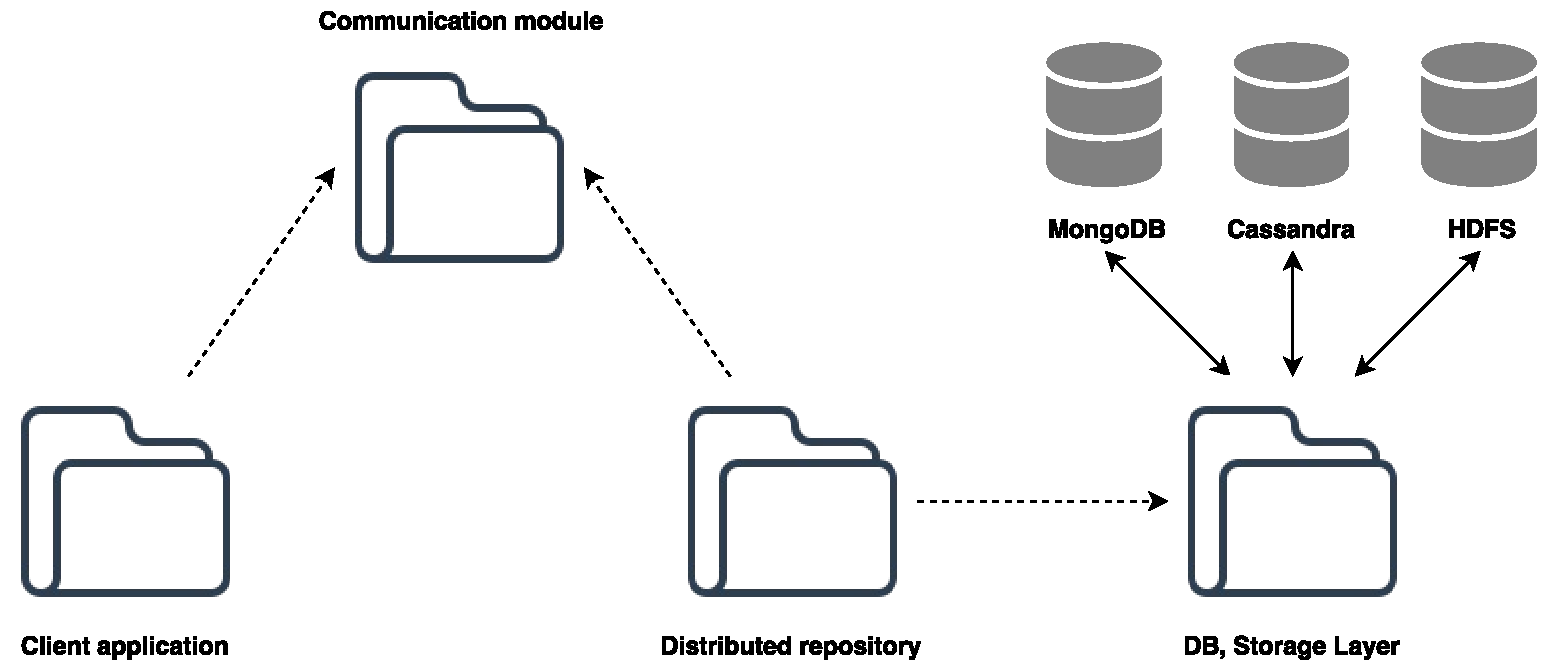
\includegraphics[width=10cm]{img/Module_dependency.pdf}
  \label{FIG_PerformanceChart}
\end{figure}
\end{frame}

%-------------------------------------

%-------------------------------------

\begin{frame}\frametitle{Prototyp}
\begin{block}{Implementace ověřující}
    \begin{itemize}
        \item Základní aspekty návrhu
        \item Konfiguraci technologií
        \item Komunikaci s klientem
        \item Výkon
    \end{itemize}
\end{block}

\begin{figure}[!h]
  \centering
  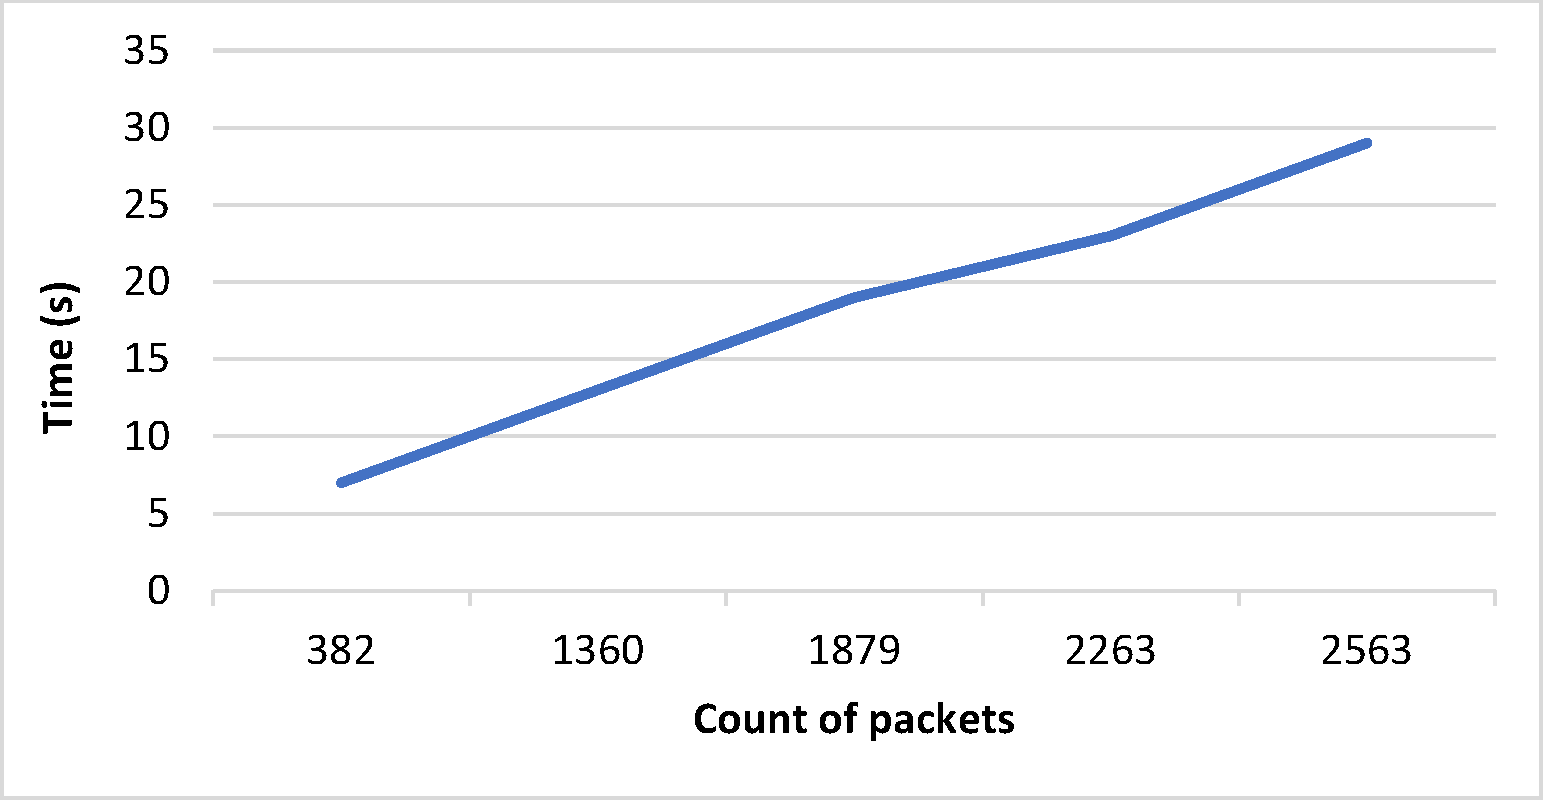
\includegraphics[width=8cm]{img/PerformanceChart.pdf}
  \label{FIG_PerformanceChart}
\end{figure}
\end{frame}

%-------------------------------------

\begin{frame}\frametitle{Další vývoj v rámci DIP}
\begin{block}{Implementace a vyhodnocení}
    \begin{itemize}
        \item Rozšíření prototypu
        \item Podsystém metadat
        \item Optimální přístup k datům
        \item Vyhodnocení z hlediska výkonu
    \end{itemize}
\end{block}
\end{frame}

%-------------------------------------

\bluepage{Děkuji za pozornost.}

\end{document}
